%%%%%%%%%%%%%%%%%%%%%%%%%%%%%%%%%%%%%%%%%
% Simple Sectioned Essay Template
% LaTeX Template
%
% This template has been downloaded from:
% http://www.latextemplates.com
%
% Note:
% The \lipsum[#] commands throughout this template generate dummy text
% to fill the template out. These commands should all be removed when 
% writing essay content.
%
%%%%%%%%%%%%%%%%%%%%%%%%%%%%%%%%%%%%%%%%%

%----------------------------------------------------------------------------------------
%	PACKAGES AND OTHER DOCUMENT CONFIGURATIONS
%----------------------------------------------------------------------------------------

\documentclass[12pt]{article} % Default font size is 12pt, it can be changed here

\usepackage{geometry} % Required to change the page size to A4
\geometry{a4paper} % Set the page size to be A4 as opposed to the default US Letter

\usepackage{graphicx} % Required for including pictures

\usepackage{float} % Allows putting an [H] in \begin{figure} to specify the exact location of the figure
\usepackage{wrapfig} % Allows in-line images such as the example fish picture


\usepackage{lipsum} % Used for inserting dummy 'Lorem ipsum' text into the template

\linespread{1.2} % Line spacing

%\setlength\parindent{0pt} % Uncomment to remove all indentation from paragraphs

\graphicspath{{./Pictures/}} % Specifies the directory where pictures are stored

\begin{document}

%----------------------------------------------------------------------------------------
%	TITLE PAGE
%----------------------------------------------------------------------------------------

\begin{titlepage}

\newcommand{\HRule}{\rule{\linewidth}{0.5mm}} % Defines a new command for the horizontal lines, change thickness here

\center % Center everything on the page

\textsc{\LARGE University Name}\\[1.5cm] % Name of your university/college
\textsc{\Large Major Heading}\\[0.5cm] % Major heading such as course name
\textsc{\large Minor Heading}\\[0.5cm] % Minor heading such as course title

\HRule \\[0.4cm]
{ \huge \bfseries Title}\\[0.4cm] % Title of your document
\HRule \\[1.5cm]

\begin{minipage}{0.4\textwidth}
\begin{flushleft} \large
\emph{Author:}\\
John \textsc{Smith} % Your name
\end{flushleft}
\end{minipage}
~
\begin{minipage}{0.4\textwidth}
\begin{flushright} \large
\emph{Supervisor:} \\
Dr. James \textsc{Smith} % Supervisor's Name
\end{flushright}
\end{minipage}\\[4cm]

{\large \today}\\[3cm] % Date, change the \today to a set date if you want to be precise

%\includegraphics{Logo}\\[1cm] % Include a department/university logo - this will require the graphicx package

\vfill % Fill the rest of the page with whitespace

\end{titlepage}

%----------------------------------------------------------------------------------------
%	TABLE OF CONTENTS
%----------------------------------------------------------------------------------------

\tableofcontents % Include a table of contents

\newpage % Begins the essay on a new page instead of on the same page as the table of contents 

%----------------------------------------------------------------------------------------
%	INTRODUCTION
%----------------------------------------------------------------------------------------

\section{Introduction} % Major section

Example citation \cite{Figueredo:2009dg}.

%------------------------------------------------

\subsection{Subsection 1} % Sub-section

\lipsum[1] % Dummy text

%------------------------------------------------

\subsection{Subsection 2} % Sub-section

\lipsum[2] % Dummy text

%------------------------------------------------

\subsubsection{Subsubsection 1} % Sub-sub-section

\lipsum[3] % Dummy text

\begin{figure}[H] % Example image
\center{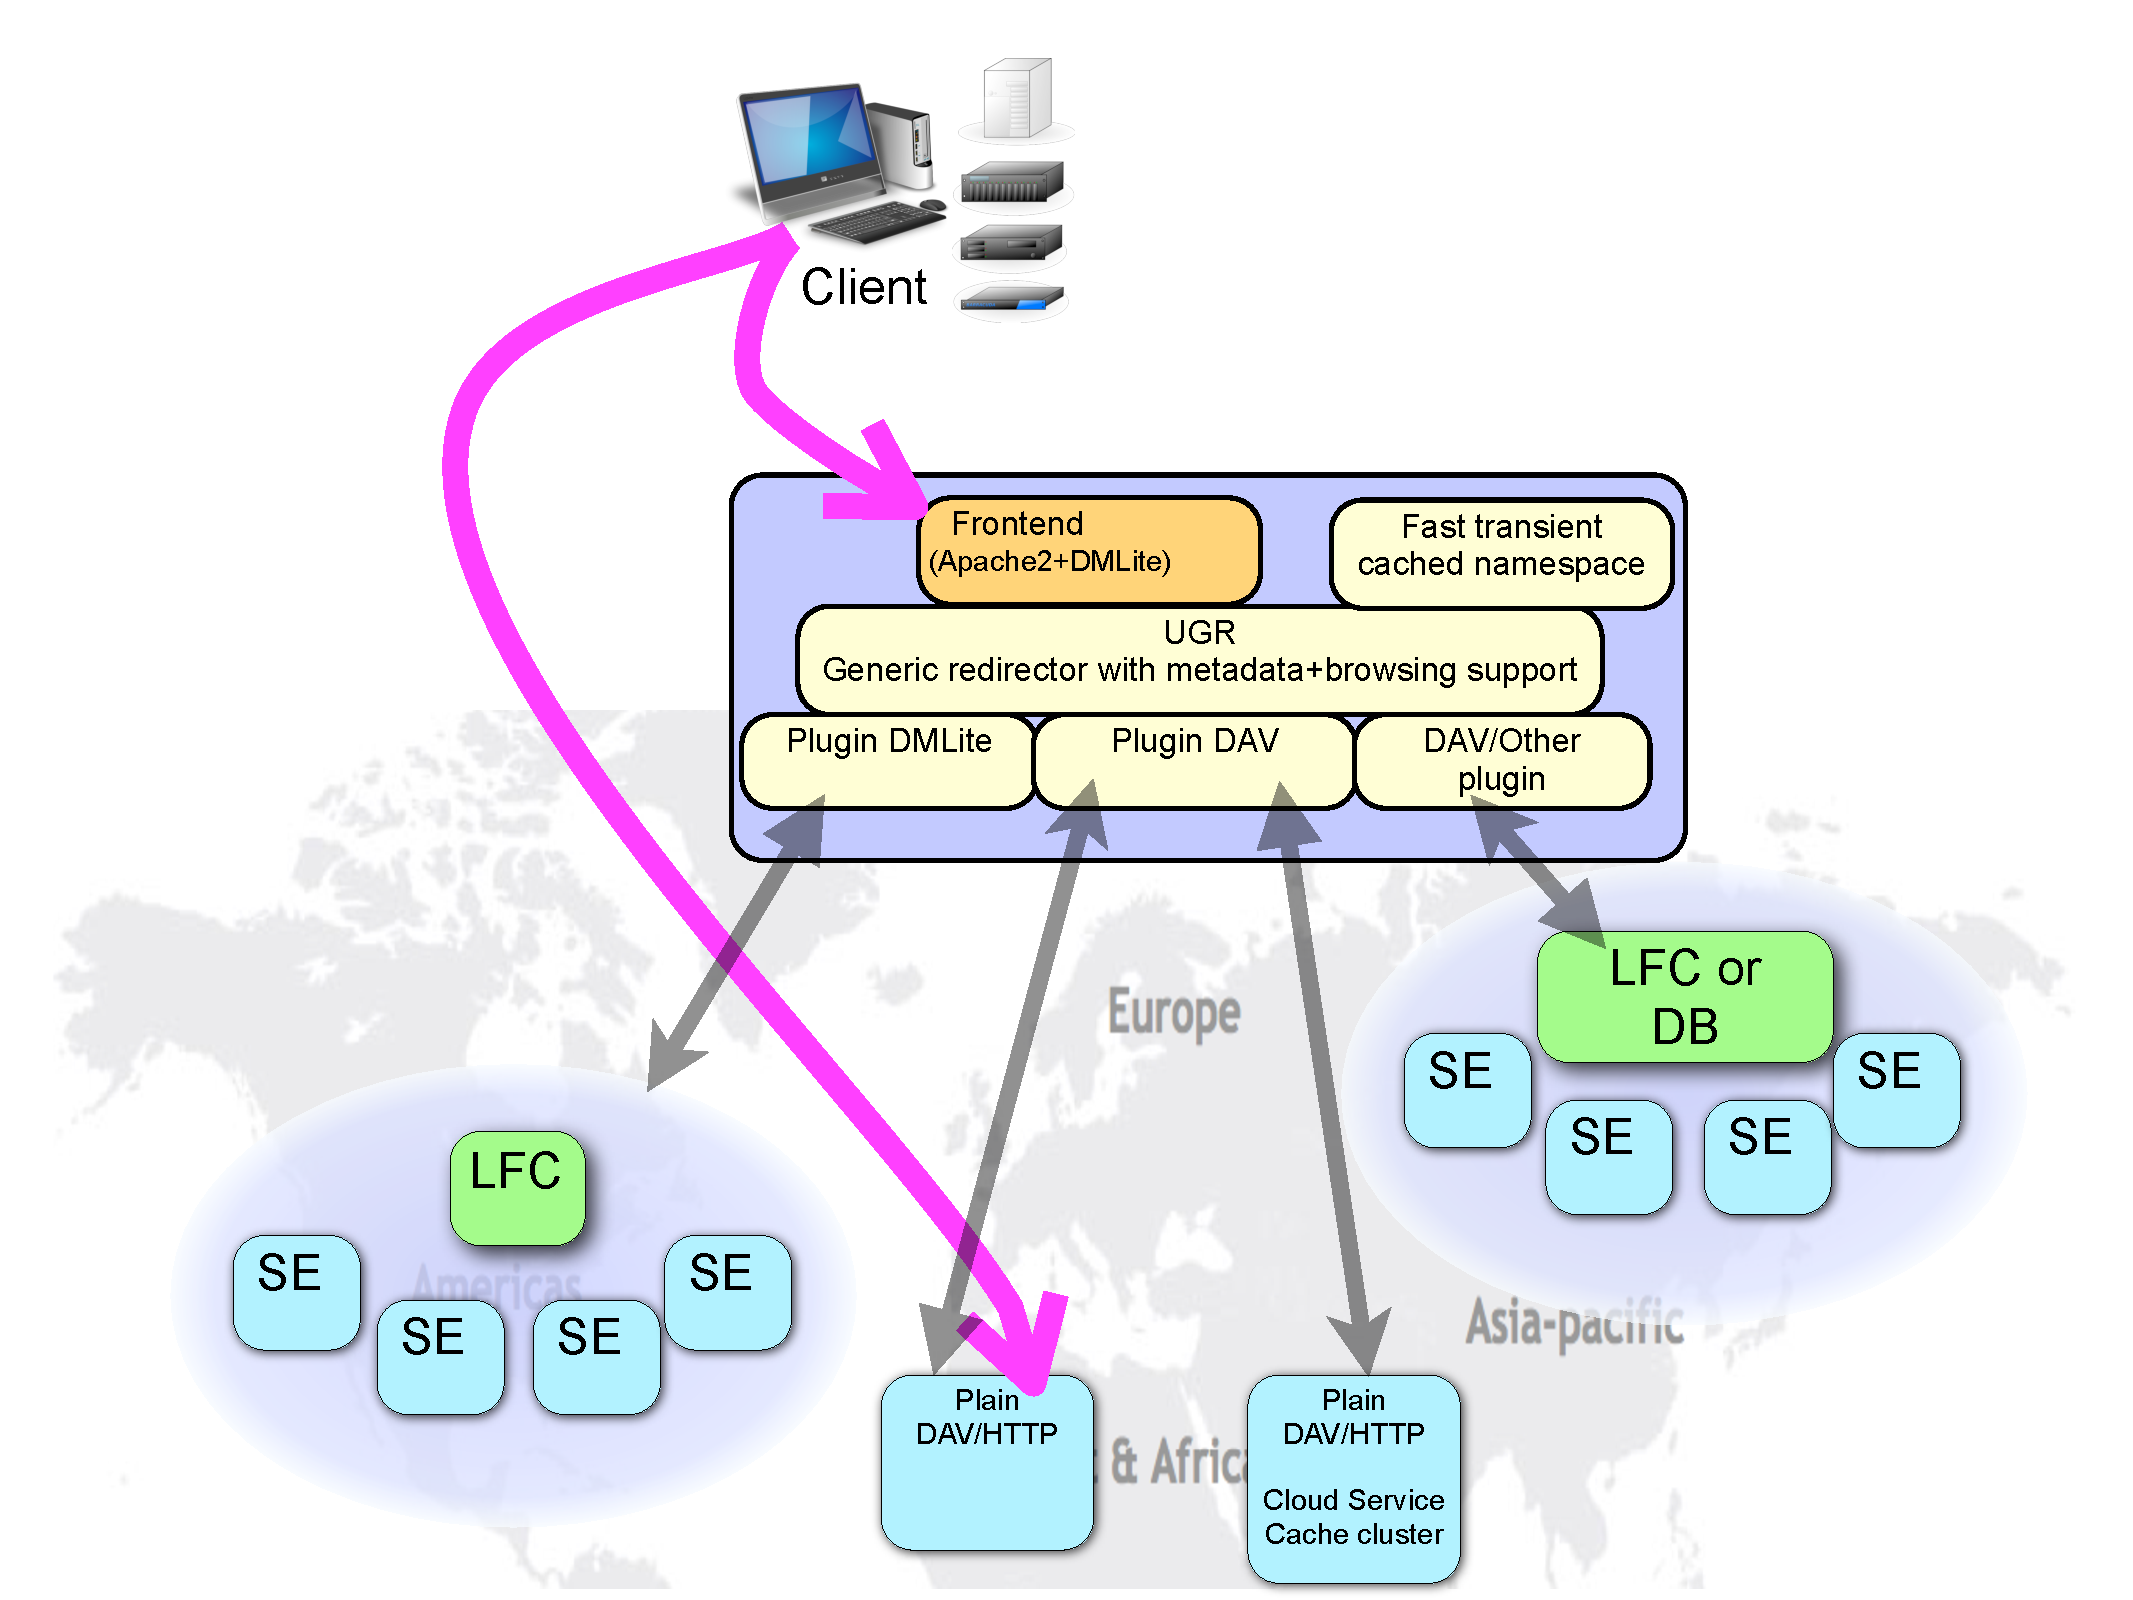
\includegraphics[width=0.5\linewidth]{dynafeds.eps}}
\caption{Example image.}
\label{fig:speciation}
\end{figure}

%------------------------------------------------

\subsubsection{Subsubsection 2} % Sub-sub-section

\lipsum[4] % Dummy text

%----------------------------------------------------------------------------------------
%	MAJOR SECTION 1
%----------------------------------------------------------------------------------------

\section{Content Section} % Major section

\lipsum[5] % Dummy text

%------------------------------------------------

\subsection{Subsection 1} % Sub-section

\subsubsection{Subsubsection 1} % Sub-sub-section

\lipsum[6] % Dummy text

%------------------------------------------------

\subsubsection{Subsubsection 2} % Sub-sub-section

\lipsum[6] % Dummy text
\begin{wrapfigure}{l}{0.4\textwidth} % Inline image example
  \begin{center}
    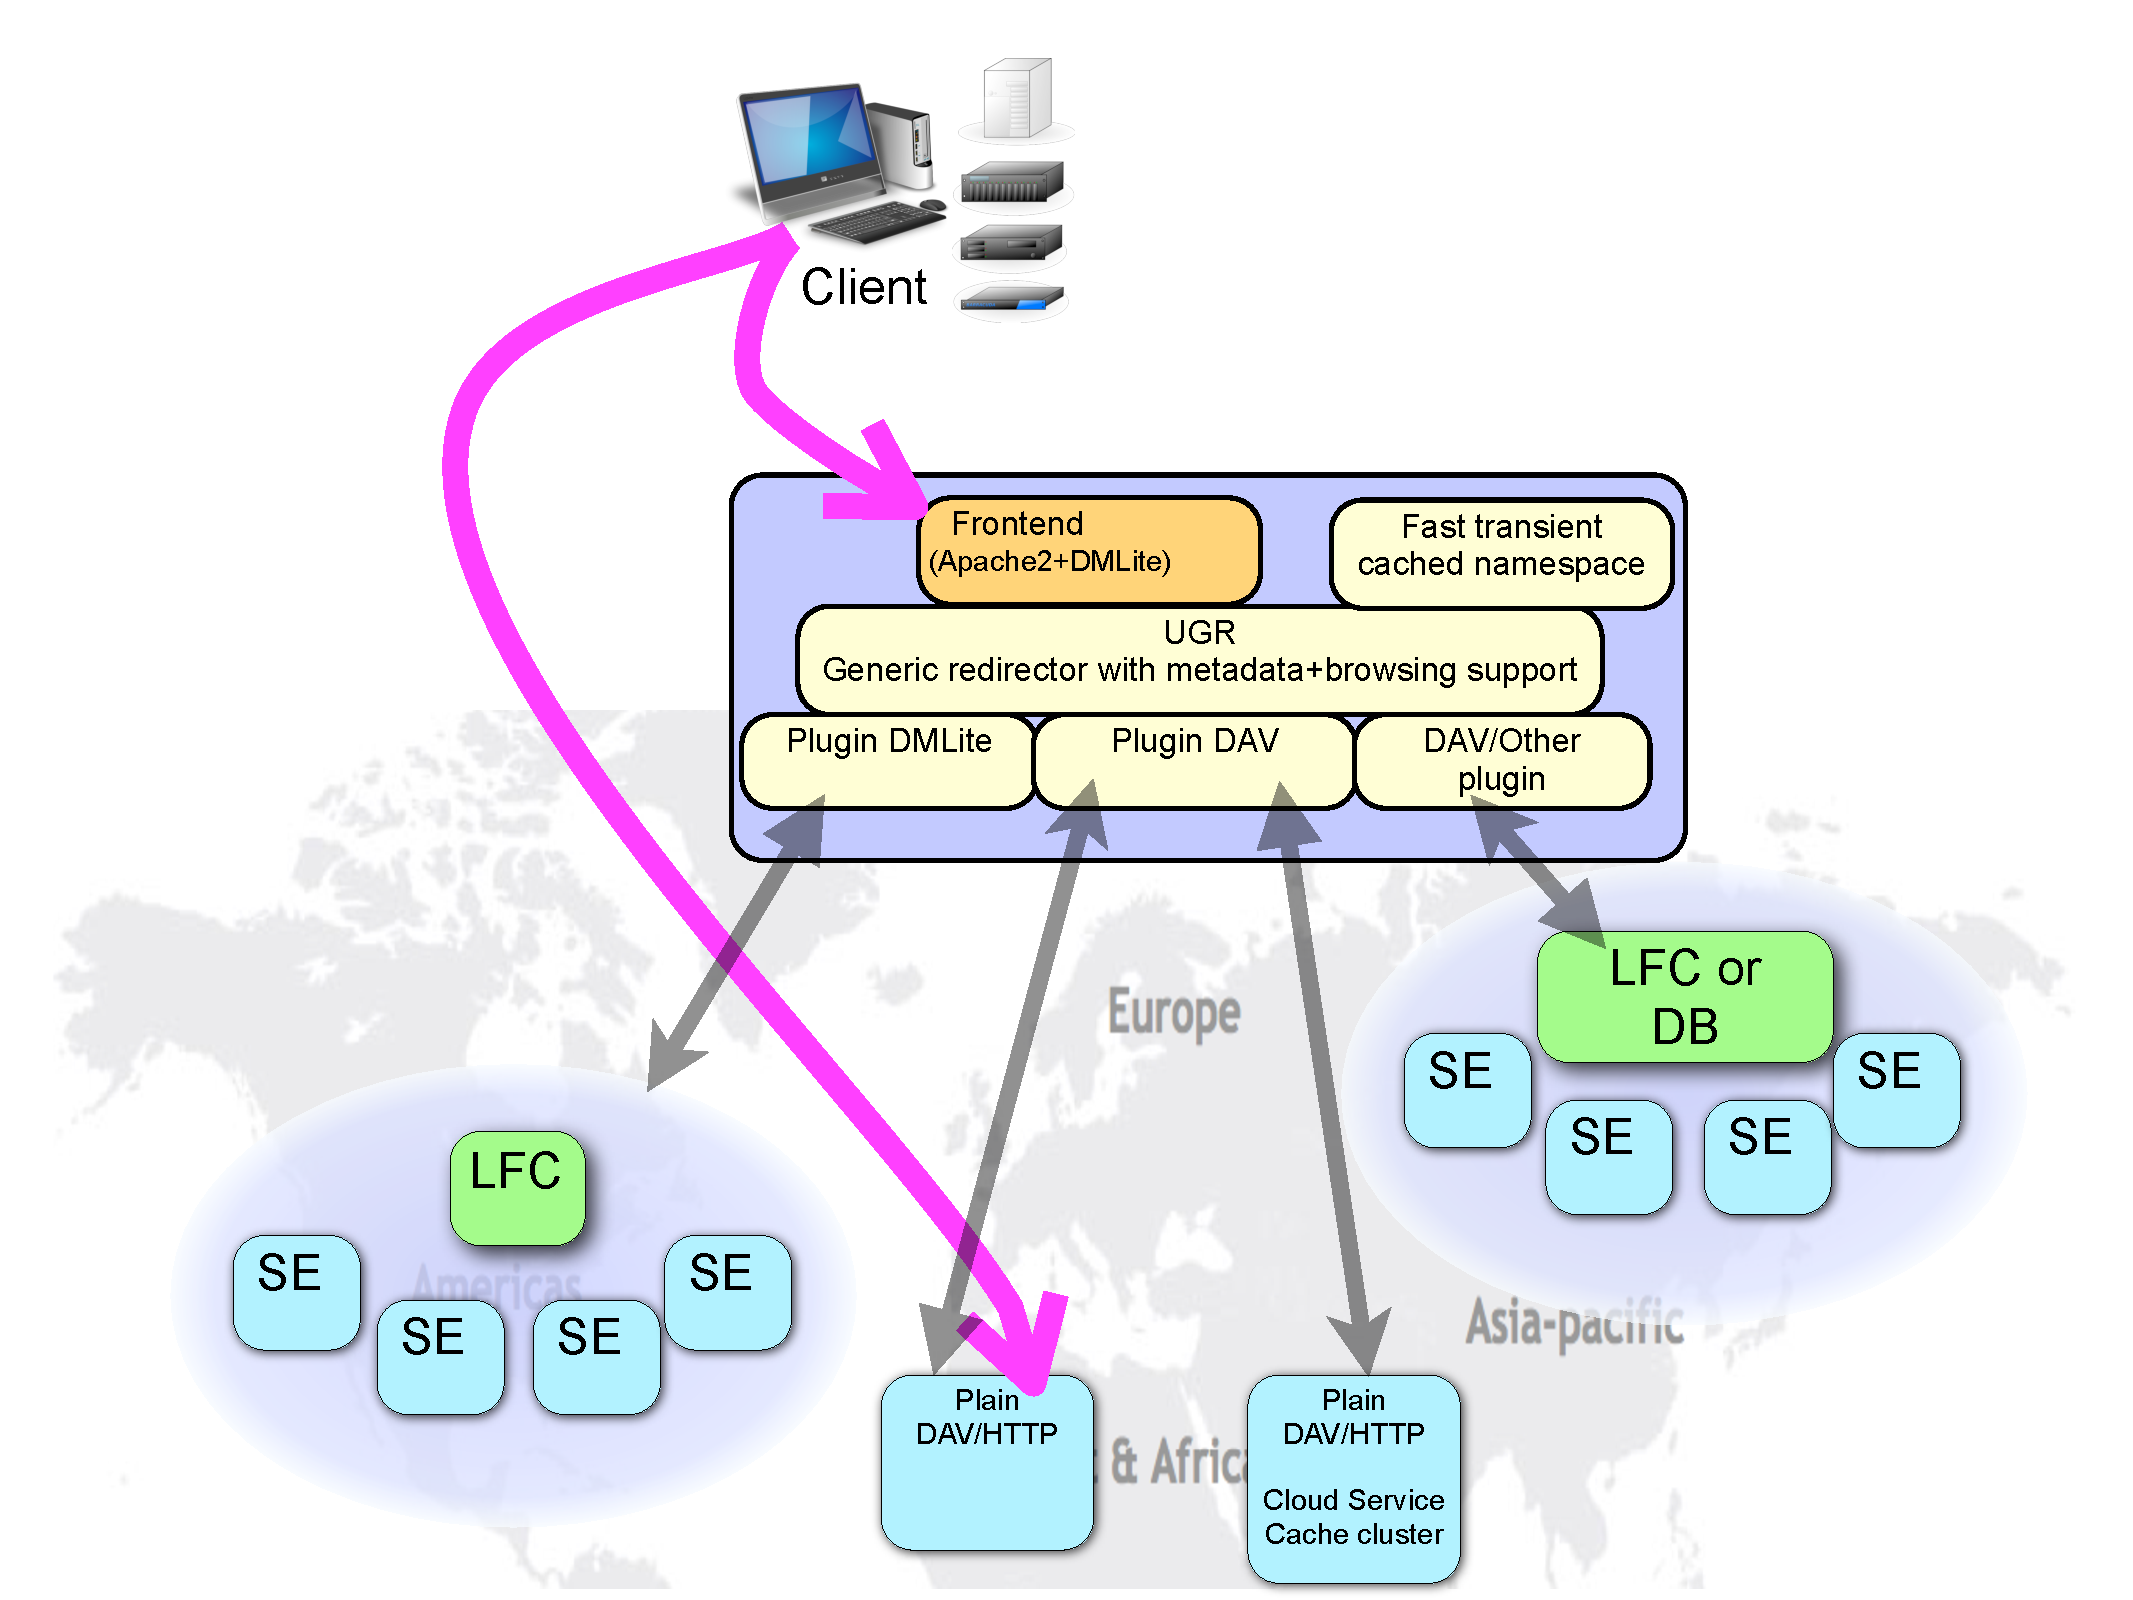
\includegraphics[width=0.38\textwidth]{dynafeds.eps}
  \end{center}
  \caption{Fish}
\end{wrapfigure}
\lipsum[7-8] % Dummy text

%------------------------------------------------

\subsubsection{Subsubsection 3} % Sub-sub-section

\begin{description} % Numbered list example

\item[First] \hfill \\
\lipsum[9] % Dummy text

\item[Second] \hfill \\
\lipsum[10] % Dummy text

\item[Third] \hfill \\
\lipsum[11] % Dummy text

\end{description} 

%----------------------------------------------------------------------------------------
%	MAJOR SECTION X - TEMPLATE - UNCOMMENT AND FILL IN
%----------------------------------------------------------------------------------------

%\section{Content Section}

%\subsection{Subsection 1} % Sub-section

% Content

%------------------------------------------------

%\subsection{Subsection 2} % Sub-section

% Content

%----------------------------------------------------------------------------------------
%	CONCLUSION
%----------------------------------------------------------------------------------------

\section{Conclusion} % Major section

\lipsum[12-13]

%----------------------------------------------------------------------------------------
%	BIBLIOGRAPHY
%----------------------------------------------------------------------------------------

\begin{thebibliography}{99} % Bibliography - this is intentionally simple in this template

\bibitem[Figueredo and Wolf, 2009]{Figueredo:2009dg}
Figueredo, A.~J. and Wolf, P. S.~A. (2009).
\newblock Assortative pairing and life history strategy - a cross-cultural
  study.
\newblock {\em Human Nature}, 20:317--330.
 
\end{thebibliography}

%----------------------------------------------------------------------------------------

\end{document}